%% chapter8_slides.tex  -  Chapter 8: Two Applications
%% The Krasnosel'skii-Mann Iterative Method: Recent Progress and Applications
%% Dong, Cho, He, Pardalos & Rassias -- SpringerBriefs in Optimization, 2022
%% Compile: pdflatex -interaction=nonstopmode chapter8_slides.tex  (twice)
\documentclass[aspectratio=169,10pt]{beamer}

\usetheme{Madrid}
\usecolortheme{seahorse}
\usefonttheme{professionalfonts}

%% packages
\usepackage{amsmath,amssymb,mathtools}
\usepackage{mathrsfs}
\usepackage{bm}
\usepackage{graphicx}
\usepackage{booktabs}
\usepackage{array}
\usepackage{listings}
\usepackage{xcolor}
\usepackage{tikz}
\usetikzlibrary{arrows.meta,positioning,shapes.geometric,fit}

\graphicspath{{figures/}}

%% listings style
\definecolor{codegray}{rgb}{0.95,0.95,0.95}
\lstdefinestyle{pycode}{
  language=Python,
  basicstyle=\ttfamily\scriptsize,
  keywordstyle=\color{blue!60!black}\bfseries,
  commentstyle=\color{green!50!black}\itshape,
  stringstyle=\color{orange!80!black},
  numbers=left,
  numberstyle=\tiny\color{gray},
  numbersep=5pt,
  frame=single,
  backgroundcolor=\color{gray!7},
  tabsize=2,
  showstringspaces=false,
  breaklines=true,
  captionpos=b,
}
\lstset{style=pycode}

%% custom colours
\definecolor{myblue}{RGB}{33,102,172}
\definecolor{myorange}{RGB}{214,96,77}
\definecolor{mygreen}{RGB}{26,152,80}

%% footline / navigation
\setbeamertemplate{footline}[frame number]
\setbeamertemplate{navigation symbols}{}

%% macros
\newcommand{\R}{\mathbb{R}}
\newcommand{\calH}{\mathcal H}
\newcommand{\Hsp}{\mathcal H}
\newcommand{\Fix}{\operatorname{Fix}}
\newcommand{\Id}{\operatorname{Id}}
\newcommand{\iprod}[2]{\langle #1, #2 \rangle}
\newcommand{\norm}[1]{\lVert #1 \rVert}

%%=============================================================================
\title[KM Method -- Ch.8]{The Krasnosel'ski\u{i}-Mann Iterative Method}
\subtitle{Chapter 8: Two Applications}
\author{Based on Dong, Cho, He, Pardalos \& Rassias}
\date{}

%%=============================================================================
\begin{document}

\begin{frame}
  \titlepage
\end{frame}

\begin{frame}{Chapter Outline}
  \tableofcontents
\end{frame}

%%=============================================================================
\section{Recap and Coordinate Decomposition}
%%=============================================================================

\begin{frame}[allowframebreaks]{Notation You'll Need / Recap}

This chapter is about \emph{scaling up} the Krasnosel'ski\u{i}--Mann (KM) iteration you already know to problems where the unknown $x$ lives in a huge-dimensional (or even infinite-dimensional) space $\Hsp$, so large that updating \emph{all} of $x$ at every step is too expensive. The trick: split $x$ into blocks and update one block ("coordinate") at a time.

\begin{block}{Recap: The KM Iteration and Averaged Operators (Ch.~3--4)}
For a nonexpansive operator $T:\Hsp\to\Hsp$ (i.e.\ $\norm{T(x)-T(y)}\le \norm{x-y}$ for all $x,y$) with $\Fix(T)\neq\emptyset$ (the fixed-point set is nonempty), write $S := \Id - T$. Then
\[
  \text{Find } x^*\in\Hsp \text{ such that } T(x^*)=x^* \qquad\Longleftrightarrow\qquad \text{Find } x^*\in\Hsp \text{ such that } S(x^*)=0.
\]
With a constant relaxation parameter $\lambda_n\equiv\lambda\in(0,1)$, the KM iteration $x_{n+1}=(1-\lambda)x_n+\lambda T(x_n)$ can be rewritten equivalently as
\[
  x_{n+1} = x_n - \lambda S(x_n) \qquad \text{for each } n\ge 0.
\]
This is the form we build on in this chapter: at each step we move $x_n$ by $-\lambda$ times the ``residual'' $S(x_n)$.
\end{block}

\begin{block}{Notation}
\begin{itemize}
  \item $\Hsp$ (calligraphic H) is a Hilbert space; $\Id$ is the identity operator, $\Id(x)=x$.
  \item $S=\Id-T$ measures how far $T$ moves a point; $S(x^*)=0$ exactly when $x^*$ is a fixed point of $T$.
  \item $\lambda$ (lambda) is the relaxation parameter from Chapter 7 --- it controls step size and can be tuned for faster convergence.
\end{itemize}
\end{block}

\framebreak

\begin{alertblock}{The Big Idea of Chapter 8: Coordinate Splitting}
Instead of moving the whole point $x\in\Hsp$ at once, split it into $m$ blocks $x=(x_1,\ldots,x_m)$ and update just \emph{one block} $x_i$ at a time --- cycling through all of them in a fixed order (\textbf{cyclic}), or letting different processors update different blocks in parallel/at random without waiting for each other (\textbf{asynchronous parallel}). This is exactly what you do with coordinate descent for a huge linear system: instead of solving for every variable simultaneously, you update $x_1$, then $x_2$, then $x_3,\ldots$, one at a time, and it still converges to the solution.
\end{alertblock}

\begin{block}{Block/Coordinate Decomposition}
Let $\Hsp_1,\ldots,\Hsp_m$ be Hilbert spaces and $\Hsp := \Hsp_1\times\cdots\times\Hsp_m$ their Cartesian product. Write $x=(x_1,\ldots,x_m)\in\Hsp$ with $x_i\in\Hsp_i$ the $i$-th \emph{block} (or \emph{coordinate}) of $x$. For $S=\Id-T:\Hsp\to\Hsp$, the $i$-th \emph{coordinate operator} is
\[
  S_i(x) := \bigl(0,\ldots,0,\, (S(x))_i,\, 0,\ldots,0\bigr) \qquad \text{for all } x\in\Hsp,
\]
i.e.\ $S_i(x)$ keeps only the $i$-th block of $S(x)$ and zeroes out every other block. Updating $x$ by $-\lambda S_i(x)$ therefore changes \emph{only} $x_i$, leaving every other block untouched.
\end{block}

\begin{block}{Cyclic Order vs.\ Asynchronous Parallel}
\begin{itemize}
  \item \textbf{Cyclic:} a single process visits coordinates $1,2,\ldots,m$ in a fixed order (or a permutation chosen once), applying one coordinate update per step; one full pass through all $m$ coordinates is called an \emph{epoch}.
  \item \textbf{Asynchronous parallel:} several agents (processors) update different coordinates \emph{concurrently, without waiting for one another}. Because agent updates interleave unpredictably, an agent may read a \emph{stale} (slightly out-of-date, or delayed) copy of the coordinates it does not own --- it does not see the very latest values written by other agents. The maximum number of such missed updates is a \emph{delay} $\tau$.
\end{itemize}
\end{block}

\end{frame}

%%=============================================================================
\section{8.1 The Asynchronous Parallel Coordinate Updates Method}
%%=============================================================================

\begin{frame}[allowframebreaks]{8.1 Why Asynchronous Parallel Updates?}

Synchronous parallel algorithms make all processors update simultaneously and then force everyone to wait at a barrier before the next round starts --- the slowest processor holds everyone else back. The \emph{asynchronous parallel} approach removes the barrier: every agent runs continuously with little idling, and iterations become \emph{disordered} (an agent may update a coordinate without having the newest information about the other coordinates).

\begin{block}{Why This Matters}
\begin{itemize}
  \item Async-parallel iteration was first introduced by Chazan and Miranker (1969) and has since been applied to linear systems, nonlinear problems, differential equations, consensus problems, and optimization.
  \item Async-parallel systems are easy to extend with new agents on the fly, and are more tolerant of computing faults and communication glitches than synchronous systems (no single point that everyone must wait on).
  \item Peng et al.\ introduced \textbf{ARock}, an algorithmic framework for asynchronous parallel coordinate updates for the fixed-point problem of nonexpansive mappings --- ARock is itself an important application of the KM iteration.
\end{itemize}
\end{block}

\begin{block}{Setting}
Let $\Hsp_1,\ldots,\Hsp_m$ be Hilbert spaces, $\Hsp:=\Hsp_1\times\cdots\times\Hsp_m$. For a nonexpansive $T:\Hsp\to\Hsp$, consider the fixed-point problem
\[
  \text{Find } x^*\in\Hsp \text{ such that } T(x^*)=x^*. \tag{8.1}
\]
As before, $S=\Id-T$ turns this into finding a zero of $S$: $0=S(x^*)$.
\end{block}

\framebreak

\begin{block}{The ARock Coordinate Update}
Let $(p_1,\ldots,p_m)$ be a probability distribution ($p_i>0$, $\sum_i p_i=1$). At step $n$, a coordinate $i_n\in\{1,\ldots,m\}$ is randomly selected with $\mathrm{Prob}(i_n=i)=p_i$, and only $x_{i_n}\in\Hsp_{i_n}$ is updated:
\[
  x_{n+1} = x_n - \frac{\eta_n}{m\,p_{i_n}}\, S_{i_n}(\hat x_n) \qquad \text{for each } n\ge 0, \tag{8.3}
\]
where $\eta_n>0$ is a scalar step size and $mp_{i_n}$ normalizes for nonuniform selection probabilities. In the \emph{uniform} case $p_i\equiv 1/m$, we have $mp_{i_n}\equiv 1$, and (8.3) simplifies to
\[
  x_{n+1} = x_n - \eta_n S_{i_n}(\hat x_n) \qquad \text{for each } n\ge 0. \tag{8.4}
\]
\end{block}

\begin{block}{Notation}
\begin{itemize}
  \item $x_n$ is the state of $x$ in \emph{global memory} just before update (8.3) is applied.
  \item $\hat x_n$ is what an agent actually \emph{reads} from global memory into its local cache and applies $S_{i_n}$ to. In a \emph{synchronous}-parallel algorithm $\hat x_n = x_n$ exactly; in ARock, because other agents may write to $x$ concurrently, $\hat x_n$ can differ from $x_n$ --- this staleness is the key difference between sync- and async-parallel algorithms.
\end{itemize}
\end{block}

\begin{block}{Quantifying the Staleness (Delay)}
The relationship between $\hat x_n$ and $x_n$ is
\[
  \hat x_n = x_n + \sum_{d\in J(n)} \bigl(x^d - x^{d+1}\bigr) \qquad \text{for each } n\ge 1, \tag{8.5}
\]
where $J(n)\subseteq\{n-1,\ldots,n-\tau\}$ and $\tau\in\mathbb N^+$ is the \emph{maximum delay}: the maximum number of other updates to $x$ that can occur during the computation of a single update (8.3). Larger $\tau$ means more staleness is tolerated, at the cost of a more delicate convergence analysis.
\end{block}

\end{frame}

\begin{frame}[allowframebreaks]{8.1 Algorithm 9 (ARock): Step by Step}

\begin{alertblock}{Intuition}
Think of $m$ workers, each responsible for one block of coordinates. Each worker, whenever it is free, grabs a random coordinate index, reads the (possibly slightly out-of-date) values of the other coordinates it needs, computes an update, and writes it back --- all without synchronizing with anyone else.
\end{alertblock}

\begin{block}{Algorithm 9 -- ARock: Framework for Asynchronous Parallel Coordinate Updates}
\textbf{Input:} $x_0\in\Hsp$, a horizon $N>0$, a distribution $(p_1,\ldots,p_m)>0$ with $\sum_{i=1}^m p_i=1$; global iteration counter $n\leftarrow 0$.

\textbf{While} $n<N$, \textbf{every agent asynchronously does the following:}
\begin{enumerate}
  \item \textbf{Select a coordinate.} Choose $i_n\in\{1,\ldots,m\}$ at random with $\mathrm{Prob}(i_n=i)=p_i$.
  \item \textbf{Update that coordinate only.} Read the (possibly stale) local copy $\hat x_n$ and perform an update to $x_{i_n}$ according to (8.3): $x_{n+1} = x_n - \dfrac{\eta_n}{mp_{i_n}}S_{i_n}(\hat x_n)$, holding every other block fixed.
  \item \textbf{Advance the counter.} Update the global counter $n\leftarrow n+1$, and continue --- with no barrier, no waiting for other agents.
\end{enumerate}
\end{block}

\textbf{Key contrast with the cyclic version (Algorithm 10, Section 8.2):} in the cyclic algorithm every coordinate is updated exactly once per epoch, in a known order, using perfectly up-to-date information. In ARock, coordinates are updated in \emph{random}, \emph{overlapping} order across agents, and the information used, $\hat x_n$, may lag behind the true global state $x_n$ by up to $\tau$ updates --- this staleness/delay is the price paid for removing synchronization barriers.

\framebreak

\begin{block}{Two Standing Assumptions}
\begin{enumerate}
  \item \textbf{Atomic coordinate update:} a coordinate is not further broken into smaller pieces during an update --- it is written all at once (no partial/torn writes).
  \item \textbf{Bounded maximal delay $\tau$:} during any update cycle of an agent, $x$ in global memory is updated at most $\tau$ times by other agents.
\end{enumerate}
For the analysis of Algorithm 9 we further need: (a) random coordinate selection, (b) a finite maximal delay $\tau$ (not essential --- an infinite delay with a light tail is also allowed), and (c) bounded relaxation parameters (standard).
\end{block}

\begin{alertblock}{When Is This Worth It?}
The coordinate update (8.3) is only computationally worthwhile if $S_i(x)$ is much cheaper to compute than the full $S(x)$ --- e.g.\ for systems of linear equations, decentralized consensus optimization, and feasibility problems, where a single coordinate can be updated from only its neighbors' data. Otherwise, it is preferable to just apply the full KM update $x_{n+1}=x_n-\lambda S(x_n)$.
\end{alertblock}

\end{frame}

\begin{frame}[allowframebreaks]{8.1 Convergence of Algorithm 9}

\begin{block}{Probabilistic Setup}
Let $(\Omega,\mathscr F,P)$ be the underlying probability space and let $\mathscr X_n:=\sigma(x_0,\hat x_1,x_1,\ldots,\hat x_n,x_n)$ be the smallest $\sigma$-algebra generated by the history up to step $n$. Assume $p_{\min}:=\min_i p_i>0$ and that the coordinate selection is conditionally i.i.d.: $\mathrm{Prob}(i_n=i\mid \mathscr X_n)=\mathrm{Prob}(i_n=i)=p_i$.
\end{block}

\begin{block}{Lemma 8.1 (One-Step Expected-Distance Bound)}
Let $T:\Hsp\to\Hsp$ be nonexpansive with $\Fix(T)\neq\emptyset$ and $\{x_n\}$ generated by Algorithm 9. Then for any $x^*\in\Fix(T)$,
\[
\mathbb E\bigl(\norm{x_{n+1}-x^*}^2\mid\mathscr X_n\bigr) \le \norm{x_n-x^*}^2 + \frac{\gamma}{m}\sum_{d\in J(n)}\norm{x_d-x_{d+1}}^2
 + \frac{1}{m}\Bigl(\frac{|J(n)|}{\gamma}+\frac{1}{mp_{\min}}-\frac{1}{\eta_n}\Bigr)\norm{x_n-\bar x_{n+1}}^2,
\]
where $\gamma>0$ is an arbitrary constant and $\bar x_{n+1}=x_n-\eta_n S(\hat x_n)$.
\end{block}

\begin{block}{Theorem 8.1 (Weak/Strong Convergence)}
Let $T$ be nonexpansive with $\Fix(T)\neq\emptyset$. If $\eta_n\in\bigl[\eta_{\min},\ \frac{cmp_{\min}}{2\tau\sqrt{p_{\min}}+1}\bigr]$ for some $\eta_{\min}>0$ and $0<c<1$, then $\{x_n\}$ from Algorithm 9 converges weakly to a fixed point of $T$ with probability one. This becomes strong convergence if $\Hsp$ is finite-dimensional, and \emph{strong} convergence to a fixed point holds (a.s.) if $T$ is demicompact. Notably, this weak-convergence result requires only that $T$ be nonexpansive with a fixed point --- no monotonicity is needed.
\end{block}

\framebreak

\begin{alertblock}{Reading the Step-Size Bound}
In the uniform case $p_{\min}\equiv p_i\equiv 1/m$, the bound $\frac{cmp_{\min}}{2\tau\sqrt{p_{\min}}+1}$ simplifies to $\frac{1}{1+2\tau/\sqrt m}$. If the maximal delay is no larger than the square root of the number of coordinates, i.e.\ $\tau=O(\sqrt m)$, the bound is $O(1)$ --- a healthy, non-shrinking step size is allowed even with many agents.
\end{alertblock}

\begin{block}{Theorem 8.2 (Linear Convergence under Quasi-Strong Monotonicity)}
Assume $S$ is quasi-$\mu$-strongly monotone with $\mu>0$ (this holds, e.g., for the KM operators arising from minimizing a closed proper convex function plus a strongly convex, Lipschitz-differentiable function). Let $\beta\in(0,1)$ and let $\{x_n\}$ be generated by Algorithm 9 with a \emph{constant} relaxation parameter $\eta\in(0,\min\{\underline\eta_1,\underline\eta_2\}]$, where
\[
  \underline\eta_1 = \Bigl(1-\frac1\rho\Bigr)\frac{m\sqrt{p_{\min}}}{8}\cdot\frac{\rho^{1/2}-1}{\rho^{(\tau+1)/2}-1} \ \text{ for some } \rho>1,
  \qquad
  \underline\eta_2 = \frac{-b+\sqrt{b^2+4(1-\beta)a}}{2a},
\]
\[
  a = \frac{2\beta\mu\tau}{m^2p_{\min}}\cdot\frac{\rho(\rho^\tau-1)}{\rho-1}, \qquad
  b = \frac{1}{mp_{\min}} + \frac2m\sqrt{\frac{\rho(\rho^\tau-1)\tau}{(\rho-1)p_{\min}}}.
\]
Then $\mathbb E(\norm{x_n-x^*}^2)\le\bigl(1-\frac{\beta\mu\eta}{m}\bigr)^n\norm{x_0-x^*}^2$, where $x^*$ is the unique fixed point of $T$.
\end{block}

\begin{alertblock}{A Clean Asymptotic Regime}
Suppose $i_n$ is uniform, $p_{\min}\equiv 1/m$, and both $m,\tau$ are large with $\sqrt\rho=1+\tfrac1\tau$. One can check $\underline\eta_1=O(\sqrt m/\tau^2)$ and $\underline\eta_2=O(\sqrt m/\tau)$. Hence if $\tau=O(m^{1/4})$, the relaxation parameter in Theorem 8.2 can be taken as $\eta=O(1)$ --- so the linear convergence rate survives even with substantial delay, as long as the delay does not grow faster than $m^{1/4}$.
\end{alertblock}

\begin{block}{Beyond ARock: Inertial Extensions}
Combining asynchronous algorithms with inertial acceleration (recall Chapters 5--6), Stathopoulos and Jones proposed an inertial asynchronous and parallel KM iteration; Heaton and Censor introduced an asynchronous sequential inertial framework for finding a point in the intersection of fixed-point sets of a finite collection of operators.
\end{block}

\end{frame}

\begin{frame}{8.1 Illustration: Cyclic vs.\ Asynchronous Schedules}

On a toy example with $m=3$ coordinates, the diagram below contrasts the two update patterns.

\begin{center}
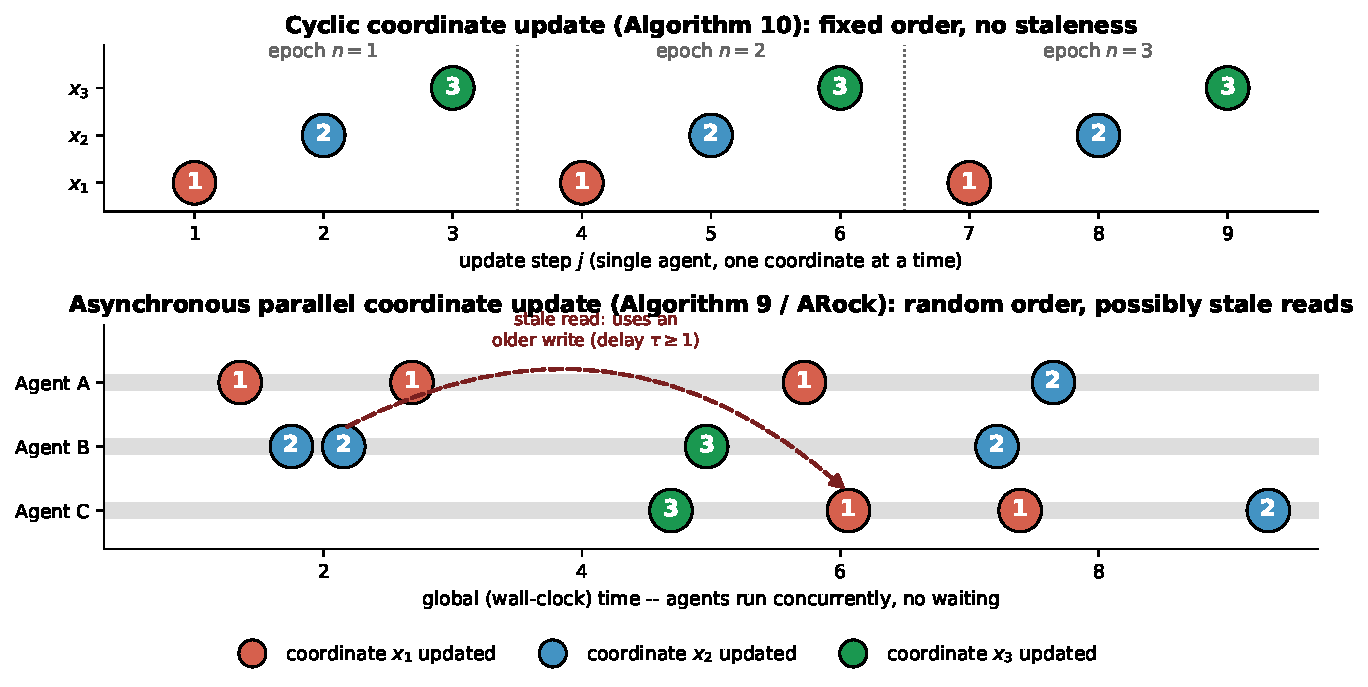
\includegraphics[width=0.85\linewidth]{fig_coordinate_updates.pdf}
\end{center}

{\footnotesize \textbf{Top:} cyclic algorithm (Sec.~8.2): coordinates $1,2,3$ in a fixed order, one sweep = one epoch, no staleness. \textbf{Bottom:} three asynchronous agents update coordinates in random order, running concurrently; the dashed arrow shows one agent using an out-of-date (stale) value because of a delay $\tau\ge 1$.}

\end{frame}

\begin{frame}[fragile]{8.1 Python (1/2): ARock-Style Async Updates -- Setup}
\begin{lstlisting}[caption={Running example and ARock scaffold (Algorithm 9)}]
import numpy as np

# Running example: A x = b (SPD, m = 3 coordinates)
A = np.array([[4., 1., 1.], [1., 4., 1.], [1., 1., 4.]])
b = np.array([6., 9., 12.])
x_star = np.linalg.solve(A, b)      # true fixed point (0.5, 1.5, 2.5)

def S(x):
    return A @ x - b                # S = Id - T (residual operator)

def arock_style(x0, n_updates, eta, tau=2, p=None, seed=0):
    """Single-machine simulation of ARock (Algorithm 9): random
    coordinate choice + a simulated stale read of size <= tau."""
    rng = np.random.default_rng(seed)
    m = len(x0)
    p = p if p is not None else np.ones(m) / m
    history = [x0.copy()]           # global memory x_0, x_1, x_2, ...
    x = x0.copy()
\end{lstlisting}
\end{frame}

\begin{frame}[fragile]{8.1 Python (2/2): ARock-Style Async Updates -- Loop}
\begin{lstlisting}[caption={ARock update loop (Steps 1--3) and usage}]
    for n in range(n_updates):
        i_n = rng.choice(m, p=p)          # Step 1: random coordinate
        delay = rng.integers(0, tau + 1)  # simulated staleness
        stale_idx = max(0, len(history) - 1 - delay)
        x_hat = history[stale_idx].copy()  # Step 2: possibly stale read
        S_i = np.zeros(m)
        S_i[i_n] = S(x_hat)[i_n]
        x = x - (eta / (m * p[i_n])) * S_i  # ARock update (8.3)
        history.append(x.copy())           # Step 3: advance counter
    return np.array(history)

hist = arock_style(np.zeros(3), n_updates=300, eta=0.2, tau=2)
print("final iterate:", hist[-1], " true x*:", x_star)
print("error:", np.linalg.norm(hist[-1] - x_star))
\end{lstlisting}
\end{frame}

%%=============================================================================
\section{8.2 The Cyclic Coordinate Update Algorithm}
%%=============================================================================

\begin{frame}[allowframebreaks]{8.2 Setup: Cyclic Coordinate Updates}

\begin{alertblock}{Intuition}
The cyclic coordinate update is the ``single-processor'' analogue of ARock: instead of a random, interleaved, possibly-stale schedule across many agents, one process visits every coordinate exactly once, in a fixed (or once-shuffled) order, always using the freshest information available. This is precisely coordinate descent / Gauss--Seidel-type sweeps, now cast in the KM framework.
\end{alertblock}

\begin{block}{Setup}
Let $T:\Hsp\to\Hsp$ be nonexpansive and $S=\Id-T$. The fixed-point problem (8.1) is equivalent to
\[
  \text{Find } x^*\in\Hsp \text{ such that } S(x^*)=0. \tag{8.6}
\]
Assume $x$ has $m$ blocks $x_i\in\Hsp_i$ for $i=1,\ldots,m$, with Cartesian product $\Hsp:=\Hsp_1\times\cdots\times\Hsp_m$. As in 8.1, the $i$-th coordinate operator is
\[
  S_i(x) = (0,\ldots,(S(x))_i,\ldots,0) \qquad \text{for all } x\in\Hsp.
\]
\end{block}

\begin{block}{Lipschitz Constants of the Coordinate Operators}
Since $T$ is nonexpansive, $S$ is $2$-Lipschitz (recall Lemma 7.3): $\norm{S(x)-S(y)}\le 2\norm{x-y}$ for all $x,y\in\Hsp$. Since $\norm{S_i(x)-S_i(y)}\le\norm{S(x)-S(y)}$, each $S_i$ is $2$-Lipschitz too --- but the Lipschitz constant of a \emph{single} coordinate operator $S_i$ can be much smaller than $2$. Denote by $L_i$ the Lipschitz constant of $S_i$:
\[
  \norm{S_i(x)-S_i(y)} \le L_i\norm{x-y} \quad \text{for all } x,y\in\Hsp, \qquad L:=\max_{1\le i\le m}L_i \le 2.
\]
$L$ will control the admissible step sizes in Theorem 8.5 below.
\end{block}

\end{frame}

\begin{frame}[allowframebreaks]{8.2 Algorithm 10: The Cyclic Coordinate Update, Step by Step}

\begin{block}{Algorithm 10 (Chow et al.) -- The Cyclic Coordinate Update}
\textbf{input:} $x_0\in\Hsp$

\textbf{for} $n=1,2,\ldots$, \textbf{do}
\begin{enumerate}
  \item \textbf{Pick an order.} Set $(i_1,i_2,\ldots,i_m)$ as a permutation of $(1,2,\ldots,m)$ (either no permutation, random shuffling, or a greedy ordering); choose a relaxation parameter $\lambda_n>0$; initialize $y_0\leftarrow x_{n-1}$.
  \item \textbf{Sweep through all $m$ coordinates.} For $j=1,2,\ldots,m$: apply the averaged-operator update to coordinate $i_j$ only, holding every other coordinate fixed,
  \[
    y_j \leftarrow y_{j-1} - \lambda_n\, S_{i_j}(y_{j-1}).
  \]
  \item \textbf{Close the epoch.} After $j=m$, set $x_n \leftarrow y_m$, and move to the next epoch $n+1$ (repeat Step 1 with a possibly new permutation).
\end{enumerate}
\end{block}

\textbf{Coordinatewise view of Step 2:} each inner iteration only touches the $i_j$-th block,
\[
  (y_j)_i = \begin{cases} (y_{j-1})_i - \lambda_n\bigl(S(y_{j-1})\bigr)_i, & \text{if } i=i_j, \\ (y_{j-1})_i, & \text{otherwise,} \end{cases} \qquad \text{for each } i=1,\ldots,m.
\]

\framebreak

\begin{block}{Notation}
\begin{itemize}
  \item $n$ indexes the \emph{outer loop} (an \emph{epoch} = one full pass through all $m$ coordinates); $j$ indexes the \emph{inner loop} (a single coordinate update within the epoch).
  \item $y_0,\ldots,y_m$ are the intermediate states within epoch $n$; $y_0$ starts from the previous epoch's result $x_{n-1}$, and $y_m$ becomes $x_n$.
  \item $\lambda_n$ is a single relaxation parameter shared by \emph{all} $m$ coordinate updates within epoch $n$ (it may change from epoch to epoch).
\end{itemize}
\end{block}

\begin{alertblock}{Choosing the Order}
The order of the $m$ coordinates is fixed at the start of each epoch, and each epoch may choose independently. Typical choices: the \emph{natural order} $(1,2,\ldots,m)$, a \emph{random shuffle}, or a \emph{greedy ordering} (placing a coordinate earlier if its Lipschitz constant $L_i$ is larger). One may also shuffle only once, at the first epoch, and reuse that order for all later epochs. In general, shuffling avoids the worst-case ordering and may accelerate convergence.
\end{alertblock}

\begin{block}{On the Relaxation Parameter}
Algorithm 10 uses the \emph{same} $\lambda_n$ for every coordinate within an epoch. But recall from Lemma 7.2 (Chapter 7) that the optimal relaxation parameter depends on the properties of the operator being applied --- so it can be beneficial to replace $\lambda_n$ by a coordinate- and epoch-dependent $\lambda_{n_{i_j}}$ instead of one shared value.
\end{block}

\end{frame}

\begin{frame}[allowframebreaks]{8.2 Convergence of Algorithm 10}

\begin{block}{Theorem 8.3 (Weak Convergence, Diminishing Step)}
Let $T:\Hsp\to\Hsp$ be nonexpansive with $\Fix(T)\neq\emptyset$. If the relaxation parameter is
\[
  \lambda_n = \frac{1}{n^{1/2}}, \tag{8.7}
\]
then the sequence $\{x_n\}$ generated by Algorithm 10 converges weakly to a fixed point of $T$.
\end{block}

\begin{block}{A Relaxed Condition (Peng and Xu)}
Condition (8.7) was relaxed to the pair of conditions
\[
  (\mathrm{G1})\ \sum_{n=0}^{+\infty}\lambda_n=+\infty \qquad \text{and} \qquad (\mathrm{G2})\ \sum_{n=0}^{+\infty}\lambda_n^3<+\infty. \tag{8.8}
\]
Condition (8.8) includes (8.7) as a special case. Note that any $\lambda_n$ satisfying (8.7) or (8.8) is decreasing and $\to 0$ as $n\to\infty$ --- this generally means \emph{slow} convergence for Algorithm 10 in this regime.
\end{block}

\begin{alertblock}{Reading (G1)--(G2)}
(G1) says the total step budget is unbounded --- the iterates can travel arbitrarily far, so they are not prevented from reaching a distant fixed point. (G2) says the steps shrink fast enough (in cube) that the sequence still settles down rather than oscillating forever. This is the same flavor of trade-off as the Robbins--Monro step-size conditions for stochastic approximation.
\end{alertblock}

\framebreak

\begin{block}{Theorem 8.4 (Residual Reduction Rate)}
Under the setting of Theorem 8.3, the reduction rate of the \emph{running minimal residual} is
\[
  \min_{j\le n}\bigl\{\norm{x_j-T(x_j)}^2\bigr\} = o\Bigl(\frac{1}{\sqrt n}\Bigr).
\]
It follows that $\min_{j\le n}\{\norm{x_j-T(x_j)}\} = o(1/n^{1/4})$.
\end{block}

\begin{block}{Theorem 8.5 (Linear Convergence, Constant Step)}
Assume $\Id-T$ is quasi-$\mu$-strongly monotone. Let $\{x_n\}$ be generated by Algorithm 10 with a constant relaxation parameter $\lambda_n\equiv\lambda$ satisfying
\[
  \lambda = \min\Bigl\{\frac{1}{4mL},\ \frac{\mu}{4\sqrt2\,mL},\ \frac{2mL}{17mL+2\mu^2}\Bigr\}. \tag{8.9}
\]
Then $\norm{x_n-x^*}^2 \le \rho^n\norm{x_0-x^*}^2$, where $\rho = 1-\frac{\lambda\mu^2}{2}<1$ and $x^*$ is the unique fixed point of $T$. When $m$ and $L/\mu$ are large, one has $\lambda = O\bigl(\frac{\mu}{mL}\bigr)$.
\end{block}

\begin{alertblock}{Diminishing vs.\ Constant Step: What to Take Away}
Theorem 8.3 needs no monotonicity but pays for it with a vanishing step size and only weak, sublinear-type guarantees (Theorem 8.4). Theorem 8.5 needs the extra structure of quasi-strong monotonicity of $\Id-T$ but rewards it with a genuinely \emph{linear} (geometric) convergence rate at a \emph{fixed} step size --- exactly the pattern you saw for relaxation parameters in Chapter 7, now applied coordinate-by-coordinate.
\end{alertblock}

\end{frame}

\begin{frame}[allowframebreaks]{8.2 Running Example: A $3\times3$ Linear System via Cyclic Updates}

\begin{alertblock}{Setting Up the Example}
Take $\Hsp=\R^3$, $m=3$ coordinates (one per scalar variable), and consider solving $Ax=b$ for a symmetric positive-definite $A$ and vector $b$:
\[
  A = \begin{pmatrix} 4 & 1 & 1 \\ 1 & 4 & 1 \\ 1 & 1 & 4 \end{pmatrix}, \qquad b = (6,\,9,\,12).
\]
Let $f(x)=\tfrac12 x^\top A x - b^\top x$ and $T(x) := x - \nabla f(x) = x-(Ax-b)$: since $A\succ 0$, $T$ is (for a suitable step) an averaged/nonexpansive operator, and its fixed points are exactly the solutions of $Ax=b$. Here $S(x)=\Id(x)-T(x) = Ax-b$ is the residual, and $S_i(x)$ keeps only the $i$-th residual component. Solving exactly, $A$ and $b$ above give the unique fixed point
\[
  x^* = (0.5,\ 1.5,\ 2.5).
\]
\end{alertblock}

\begin{block}{Choosing $\lambda_n$: Exact Coordinate Minimization (Gauss--Seidel)}
Every diagonal entry $A_{ii}=4$, so taking $\lambda_n\equiv\lambda=1/4=1/A_{ii}$ for every coordinate makes the update (Step 2 of Algorithm 10) \emph{exactly zero out} the $i$-th residual: this is precisely a Gauss--Seidel sweep,
\[
  y_j \Big|_{i=i_j} = (y_{j-1})_{i_j} - \tfrac14\bigl(A y_{j-1}-b\bigr)_{i_j} \;=\; \frac{b_{i_j}-\sum_{k\ne i_j}A_{i_j k}(y_{j-1})_k}{A_{i_j i_j}}.
\]
We use the natural order $(1,2,3)$ and start from $x_0=(0,0,0)$.
\end{block}

\framebreak

\begin{exampleblock}{Epoch 1 (by hand)}
$y_0=x_0=(0,0,0)$.
\begin{align*}
  j{=}1:\ & S(y_0)=Ay_0-b=(-6,-9,-12);\quad y_1 = y_0-\tfrac14(-6,0,0) = (1.5,\ 0,\ 0) \\
  j{=}2:\ & Ay_1-b = (0,\,-7.5,\,-10.5);\quad y_2 = y_1-\tfrac14(0,-7.5,0) = (1.5,\ 1.875,\ 0) \\
  j{=}3:\ & Ay_2-b = (1.875,\,0,\,-8.625);\quad y_3 = y_2-\tfrac14(0,0,-8.625) = (1.5,\ 1.875,\ 2.15625)
\end{align*}
So $x_1=(1.5,\ 1.875,\ 2.15625)$, with $\norm{x_1-x^*}\approx 1.122$ (down from $\norm{x_0-x^*}=\norm{(0,0,0)-(0.5,1.5,2.5)}\approx 2.958$).
\end{exampleblock}

\begin{exampleblock}{Epoch 2 (by hand)}
$y_0=x_1=(1.5,\,1.875,\,2.15625)$.
\begin{align*}
  j{=}1:\ & Ay_0-b=(4.03125,\,2.15625,\,0);\quad y_1=(0.4921875,\ 1.875,\ 2.15625) \\
  j{=}2:\ & Ay_1-b=(0,\,1.1484375,\,-1.0078125);\quad y_2=(0.4921875,\ 1.587890625,\ 2.15625) \\
  j{=}3:\ & Ay_2-b=(-0.287109375,\,0,\,-1.294921875);\quad y_3=(0.4921875,\ 1.587890625,\ 2.47998046875)
\end{align*}
So $x_2 \approx (0.4922,\ 1.5879,\ 2.4800)$, and $\norm{x_2-x^*}\approx 0.0905$ --- already within one-tenth of the fixed point after just two epochs, six coordinate updates total.
\end{exampleblock}

\framebreak

\begin{block}{Continuing the Sweep: Epochs 3--5}
\begin{center}
\begin{tabular}{crrrc}
\toprule
Epoch $n$ & $x_1$ & $x_2$ & $x_3$ & $\norm{x_n-x^*}$ \\
\midrule
0 & 0.0000 & 0.0000 & 0.0000 & 2.9580 \\
1 & 1.5000 & 1.8750 & 2.1563 & 1.1220 \\
2 & 0.4922 & 1.5879 & 2.4800 & 0.0905 \\
3 & 0.4830 & 1.5092 & 2.5019 & 0.0194 \\
4 & 0.4972 & 1.5002 & 2.5006 & 0.0029 \\
5 & 0.4998 & 1.4999 & 2.5001 & 0.0003 \\
\bottomrule
\end{tabular}
\end{center}
The error shrinks geometrically epoch over epoch --- consistent with Theorem 8.5's linear-rate guarantee (here the convergence is even faster than the generic worst case, because $\lambda=1/A_{ii}$ performs \emph{exact} coordinate minimization at each step, i.e., classical Gauss--Seidel on a diagonally dominant SPD matrix).
\end{block}

\begin{alertblock}{A Brief Aside: Connection to the Book's Projection Example}
The book's running example in earlier chapters used $P_C$, the projection onto the closed unit disk. A coordinate-update view of a projection onto a \emph{box} $C=[a_1,b_1]\times \cdots \times [a_m,b_m]$ would similarly act coordinatewise: $(P_C(x))_i = \mathrm{clip}(x_i, a_i, b_i)$, updated one $i$ at a time. We use the linear-system example here instead, since it is the more natural vehicle for illustrating coordinate splitting with concrete numbers.
\end{alertblock}

\end{frame}

\begin{frame}{8.2 Illustration: Convergence of the Cyclic Update}

\begin{center}

\includegraphics[width=0.95\linewidth]{fig_convergence.pdf}
\end{center}

{\small \textbf{Left:} the three coordinates $x_1,x_2,x_3$ converge to $x^*=(0.5,1.5,2.5)$ (dashed lines) within a handful of epochs. \textbf{Right:} the distance $\norm{x_n-x^*}$ on a log scale, showing the geometric (linear) decay predicted by Theorem 8.5.}

\end{frame}

\begin{frame}[fragile]{8.2 Python (1/2): Cyclic Coordinate Update -- Setup}
\begin{lstlisting}[caption={Running example and Algorithm 10 scaffold}]
import numpy as np

A = np.array([[4., 1., 1.], [1., 4., 1.], [1., 1., 4.]])
b = np.array([6., 9., 12.])
x_star = np.linalg.solve(A, b)          # (0.5, 1.5, 2.5)

def S(x):
    return A @ x - b                    # S = Id - T, the residual

def cyclic_coordinate_update(x0, n_epochs, lam, order=None):
    """Algorithm 10: one full cyclic sweep through all m coordinates
    is one epoch; order=None uses the natural order (1,...,m)."""
    m = len(x0)
    x = np.array(x0, dtype=float)
    history = [x.copy()]
    for n in range(1, n_epochs + 1):
        seq = order if order is not None else range(m)
        y = x.copy()
\end{lstlisting}
\end{frame}

\begin{frame}[fragile]{8.2 Python (2/2): Cyclic Coordinate Update -- Sweep}
\begin{lstlisting}[caption={Algorithm 10, Steps 2--3, and results on $Ax=b$}]
        for i in seq:                        # Step 2: sweep coordinates
            Sy = S(y)
            Si = np.zeros(m)
            Si[i] = Sy[i]                     # S_i keeps only block i
            y = y - lam * Si                  # update coordinate i only
        x = y.copy()                          # Step 3: close the epoch
        history.append(x.copy())
    return np.array(history)

lam = 1.0 / 4.0                    # = 1/A_ii (exact coord. minimization)
hist = cyclic_coordinate_update(np.zeros(3), n_epochs=5, lam=lam)
errors = np.linalg.norm(hist - x_star, axis=1)
for n, (x_n, e) in enumerate(zip(hist, errors)):
    print(f"epoch {n}: x={x_n.round(4)}, ||x_n-x*||={e:.4f}")
# epoch 0: [0. 0. 0.]             , 2.9580
# epoch 1: [1.5    1.875  2.1563] , 1.1220
# epoch 2: [0.4922 1.5879 2.48  ] , 0.0905   -> x* = [0.5 1.5 2.5]
\end{lstlisting}
\end{frame}

%%=============================================================================
\section{Conclusion: Where This Leaves Us}
%%=============================================================================

\begin{frame}[allowframebreaks]{Conclusion: Where This Leaves Us}

\begin{block}{The Book's Own Conclusion (verbatim themes)}
``The Krasnosel'ski\u{i}--Mann iteration is the most popular algorithm to solve the fixed point problems. Its role in the construction and analysis of the iterative algorithms, especially operator splitting methods, in optimization has recently paid increasing attention. Relaxation and inertia are two main factors that affect the convergence speed of the Krasnosel'ski\u{i}--Mann iteration. Although some progress has been made on the range and selections of the inertial and relaxation parameters, there are few results on the optimal choices. Much of the space remains to be explored for the Krasnosel'ski\u{i}--Mann iteration.''
\end{block}

\begin{alertblock}{Two Open Problems the Book Leaves Us With}
\begin{itemize}
  \item There is still no complete theory for the \emph{optimal} choice of relaxation parameters $\lambda_n$ (Chapter 7) or inertial parameters (Chapters 5--6) --- only ranges and sufficient conditions are known.
  \item Much of the design space of KM-type methods (how to combine relaxation, inertia, and coordinate splitting) remains unexplored, especially in the large-scale / distributed regime studied in this chapter.
\end{itemize}
\end{alertblock}

\framebreak

\begin{block}{The Arc of the Whole Book, in One Slide}
\begin{enumerate}
  \item \textbf{Ch.~3 -- The KM iteration.} $x_{n+1}=(1-\lambda_n)x_n+\lambda_n T(x_n)$ for nonexpansive $T$: the basic machine for finding fixed points, with weak convergence under mild conditions.
  \item \textbf{Ch.~4 -- Operator splitting as KM.} Forward--backward, Douglas--Rachford, ADMM, and other splitting methods are all revealed to be instances of the KM iteration for a suitably built nonexpansive operator --- a unifying lens.
  \item \textbf{Ch.~5 -- Inertial KM.} Adding a momentum/inertial term accelerates convergence, echoing Nesterov-type acceleration in smooth convex optimization.
  \item \textbf{Ch.~6 -- Multi-step inertial KM.} Using several past iterates (not just one) for the inertial term, generalizing Chapter 5's single-step inertia.
  \item \textbf{Ch.~7 -- Relaxation parameters.} How to choose (and adapt) $\lambda_n$ to speed up convergence, with sharper rates under extra structure (e.g.\ strong monotonicity).
  \item \textbf{Ch.~8 -- Coordinate-update applications (this chapter).} Cyclic and asynchronous-parallel coordinate updates let the whole KM framework scale to problems where $x$ has millions of coordinates and updating all of them at once is infeasible.
\end{enumerate}
\end{block}

\begin{alertblock}{Takeaway}
Every method in this book, from the plain KM iteration to ARock's asynchronous coordinate updates, is built from the same two ingredients: a nonexpansive operator $T$ (or its residual $S=\Id-T$) and a carefully chosen step (relaxation, inertia, or which coordinate to touch next). The frontier is tuning these ingredients optimally --- and, as the authors note, that frontier is still wide open.
\end{alertblock}

\end{frame}

\end{document}
